% Article (English version) — Relativistic Simulator (Physics 4)
% Compile with:  tectonic artigo-en.tex
\documentclass[10pt,a4paper,twocolumn]{article}

\usepackage{fontspec}            % XeTeX: Unicode
\usepackage[english]{babel}
\usepackage{amsmath}
\usepackage{amssymb}
\usepackage{geometry}
\geometry{a4paper, top=2.4cm, bottom=2.6cm, left=1.7cm, right=1.7cm, columnsep=0.65cm}
\usepackage{graphicx}
\usepackage{booktabs}
\usepackage{array}
\usepackage{caption}
\captionsetup{labelsep=period, font=small, skip=6pt}
\usepackage{titlesec}
\titleformat{\section}{\centering\normalsize}{\thesection.}{0.55em}{\MakeUppercase}
\titleformat{\subsection}{\normalsize\itshape}{\thesubsection}{0.6em}{}
\titlespacing{\section}{0pt}{14pt plus 3pt minus 2pt}{8pt plus 2pt}
\titlespacing{\subsection}{0pt}{10pt plus 3pt minus 2pt}{5pt plus 1pt}
\usepackage{tikz}
\usetikzlibrary{arrows.meta, positioning}
\usepackage[hidelinks]{hyperref}
\urlstyle{tt}

\setlength{\parskip}{0pt}
\setlength{\parindent}{1.2em}

% Author-year reference list with hanging indent
\newenvironment{referencias}
  {\section*{REFERENCES}\small
   \begin{list}{}{\setlength{\leftmargin}{1.4em}\setlength{\itemindent}{-1.4em}%
                  \setlength{\itemsep}{2pt}\setlength{\parsep}{0pt}}}
  {\end{list}}

\begin{document}

\twocolumn[{
  \begin{center}
    {\large\bfseries Relativistic Simulator: Real-Time Interactive Visualization\\[0.25em]
     of the Optical Effects of Special Relativity\,\textsuperscript{$\star$}\par}
    \vspace{1.5em}
    {\bfseries Sergio Roncato Maccari\,\textsuperscript{*}}\par
    \vspace{1.1em}
    {\small\itshape \textsuperscript{*}\,Faculdade de Engenharia de Computação, Universidade
     Tecnológica Federal do Paraná,\\ PR, Brazil (e-mail: sergiomaccari@alunos.utfpr.edu.br).}\par
  \end{center}
  \vspace{0.9em}
  \hrule height 0.4pt
  \vspace{1.0em}
  {\small
  \noindent\textbf{Abstract:} Special Relativity is usually taught through isolated formulas,
  and students rarely develop a visual intuition of how the world would actually look at
  speeds close to the speed of light. This work presents an interactive simulator, running
  in real time in the web browser (TypeScript + Three.js/WebGL), that turns the canonical
  equations of Special Relativity into a navigable 3D scene: Lorentz contraction, time
  dilation, relativistic aberration (via the past light cone), the relativistic Doppler
  effect and relativistic beaming, with color computed by spectral reconstruction based on
  CIE response curves. All the per-frame visible physics is evaluated per vertex on the GPU,
  in GLSL shaders, and the spectral-reconstruction integral is solved once on the CPU at
  start-up, which keeps the simulation interactive even on modest hardware. Three observation modes
  (orbital laboratory, observer's eye and first person at constant velocity) let the user
  separate what is \emph{measured} from what is \emph{seen}, which is the central conceptual
  distinction of relativistic optics.\par
  }
  \vspace{0.8em}
  {\small\itshape
  \noindent Keywords: Special Relativity; Scientific Visualization; WebGL; Doppler Effect;
  Computer Graphics.\par
  }
  \vspace{0.7em}
  \hrule height 0.4pt
  \vspace{1.8em}
}]

{\let\thefootnote\relax\footnotetext{$^{\star}$ Work developed in the Physics 4
course. A versão em português deste artigo está disponível no mesmo repositório
(\texttt{docs/artigo.pdf}).}}

\section{Introduction}

Special Relativity, formulated by Einstein (1905), is presented in undergraduate courses
mainly in the form of equations: length contraction, time dilation and the Doppler effect
appear as isolated formulas, verified in numerical exercises. Students rarely form a
coherent mental picture of \emph{what the world would look like} to a relativistic
traveler, partly because no everyday experience comes close to the regime $v \sim c$,
partly because the effects never occur in isolation: contraction, light propagation delay,
aberration, color shift and brightness variation are simultaneous manifestations of a
single geometric structure, Minkowski spacetime.

There is also a recurring conceptual confusion in the introductory study of Special
Relativity: treating \emph{measuring} and \emph{seeing} as synonyms. Lorentz contraction
is a fact of \emph{measurement} (the simultaneous recording, in the observer's frame, of
the two ends of an object); the \emph{image} captured by an eye or a camera, on the other
hand, combines past events, because light has a finite speed. Terrell (1959) and Penrose
(1959) showed, independently, that a fast object of small angular size does not look
flattened in a photograph, but rotated. Distinguishing these two concepts requires
visualizing the two stages separately, which is unfeasible with static figures.

Attacking this gap through interactive visualization is not a new idea, and the most
influential reference comes from the MIT Game Lab. The game \emph{A Slower Speed of Light}
(Kortemeyer et al., 2013) places the player in a world where the speed of light drops
progressively down to walking pace, and \emph{OpenRelativity} (MIT Game Lab, 2013; Sherin
et al., 2016) generalizes that engine into an open-source toolkit for the Unity engine.
These projects established what is now the canonical visual repertoire of the field, that
is, contraction, aberration, Doppler and beaming applied to a navigable scene, and they
are the acknowledged inspiration for this work. The difference in scope lies in the
execution medium and in the intended audience: OpenRelativity presupposes a Unity
installation and the compilation of a project, whereas the simulator described here was
written from scratch as a static web page, in TypeScript and GLSL on top of WebGL, which
opens in any modern browser with no installation and no dedicated hardware. The design
priority was to lower as far as possible the barrier to entry for the undergraduate
student who simply wants to see the phenomenon.

This work presents an interactive simulator that fills this gap. It is a single-page web
application, written in TypeScript on top of the Three.js library (WebGL), in which all
the relativistic physics is evaluated \emph{per vertex} on the graphics card, in GLSL
shaders. The user adjusts the fraction of the speed of light, $\beta = v/c$, and
immediately observes the combined effect (or each effect in isolation, since every effect
can be switched on and off individually) of Lorentz contraction, retarded time (apparent
position), the relativistic Doppler effect and beaming on the same three-dimensional
scene.

The physical scope was restricted to Special Relativity in the simple regime, consistent
with the Physics 4 syllabus: sources and observer move with \emph{constant velocity},
without relativistic acceleration and without General Relativity effects. This
restriction is sufficient to correctly reproduce the most striking visual phenomena of
high-speed motion, and the corresponding theoretical background (Nussenzveig, 2014;
Griffiths, 2017) is developed in Section~2. Section~3 describes the implementation
methodology (architecture, GPU algorithms and observation modes), Section~4 presents the
results and the limitations of the model, and Section~5 concludes.

\section{Theoretical Background}

\subsection{Postulates and the Lorentz transformation}

Special Relativity rests on two postulates (Einstein, 1905): (i) the laws of physics have
the same form in every inertial frame; (ii) light propagates in vacuum with the same
speed $c$ in every inertial frame, regardless of the motion of the source or of the
observer. The second postulate, imposed by the experimental evidence of Michelson and
Morley (1887), breaks with Galilean kinematics and forces a revision of the concepts of
space, time and simultaneity.

For two inertial frames $S$ and $S'$, with $S'$ moving with velocity $v$ along the $x$
axis of $S$ and origins coinciding at $t = t' = 0$, the postulates lead to the
\emph{Lorentz transformation}:
\begin{equation}
  \begin{aligned}
    t' &= \gamma\left(t - \frac{v\,x}{c^{2}}\right), \qquad &
    x' &= \gamma\,(x - v\,t),\\
    y' &= y, & z' &= z,
  \end{aligned}
  \label{eq:lorentz}
\end{equation}
with the central dimensionless quantities of the whole theory:
\begin{equation}
  \beta = \frac{v}{c} \in [0,1), \qquad
  \gamma = \frac{1}{\sqrt{1-\beta^{2}}} \geq 1.
  \label{eq:gamma}
\end{equation}
The transformation preserves the invariant interval
$s^{2} = c^{2}t^{2} - x^{2} - y^{2} - z^{2}$, which guarantees that $c$ is the same for
all observers. The simulator always works with the dimensionless velocity
$\vec{\beta} = \vec{v}/c$, so the geometry never depends explicitly on $c$; the numerical
value of $c$ only reappears when converting intervals to seconds.

\subsection{Length contraction and time dilation}

The two classic kinematic effects follow from Eq.~\eqref{eq:lorentz}. A ruler of proper
length $L_{0}$, at rest in $S'$ and aligned with the motion, has its two ends recorded
\emph{at the same instant} by an observer in $S$; the measured length is
\begin{equation}
  L = \frac{L_{0}}{\gamma} = L_{0}\sqrt{1-\beta^{2}}.
  \label{eq:contracao}
\end{equation}
A clock at rest in $S'$, marking two events separated by the proper time $\Delta\tau$, is
measured in $S$ with the dilated interval
\begin{equation}
  \Delta t = \gamma\,\Delta\tau \geq \Delta\tau .
  \label{eq:dilatacao}
\end{equation}
Both effects are displayed directly by the simulator: contraction is applied to the
geometry per vertex; dilation is shown by two analog clocks in the readout panel, with
$d\tau = dt/\gamma$ integrated every frame.

\subsection{Relativistic velocity addition}

If a particle has velocity $\vec{u}$ (in units of $c$) in a frame that, in turn, moves
with $\vec{v}$ relative to the laboratory, the composed velocity is not the Galilean sum.
Decomposing $\vec{u}$ into components parallel and perpendicular to $\vec{v}$,
\begin{equation}
  \vec{u}\,' =
  \frac{\vec{u}_{\parallel} + \vec{v} + \vec{u}_{\perp}/\gamma_{v}}
       {1 + \vec{u}\cdot\vec{v}},
  \qquad
  \gamma_{v} = \frac{1}{\sqrt{1-|\vec{v}|^{2}}}.
  \label{eq:veladd}
\end{equation}
Eq.~\eqref{eq:veladd} recovers the Galilean limit when $|\vec{u}|, |\vec{v}| \ll 1$ and
saturates at $c$: for collinear motion, $u' = (u+v)/(1+uv)$, so that $u = 1$ (light)
implies $u' = 1$ for any $v$; the second postulate is respected automatically. The factor
$1/\gamma_{v}$ in the transverse component is the geometric origin of the aberration of
light. This equation is implemented in the physics core of the simulator and replicated
in GLSL in the vertex shader, where it is evaluated vertex by vertex to compose the
velocity of each object with that of the observer, guaranteeing $|\vec{\beta}| < 1$ for
any combination.

\subsection{Measuring is not seeing: the past light cone}
\label{sec:conedeluz}

\emph{Measuring} is an idealized, simultaneous operation in the observer's frame; it is
what the Lorentz transformation describes. \emph{Seeing}, on the other hand, is capturing
at a single point, the eye, all the light rays arriving now. Since light has a finite
speed, the photons reaching the eye at this instant left different points of the source
at \emph{different instants in the past}. The image is not an instantaneous portrait, but
a stitching of events on the past light cone of the observation event.

Consider the observer at the origin, at time $t = 0$, and a source point with position
$\vec{r}$ (at $t=0$) and constant velocity $\vec{u}$ (in units of $c$). The past instant
$\tau \leq 0$ at which this point emitted the light arriving now satisfies the
\emph{retarded-time condition} $|\vec{r} + \vec{u}\,\tau| = -\tau$, which squared gives
the quadratic equation
\begin{equation}
  \bigl(|\vec{u}|^{2}-1\bigr)\,\tau^{2}
  + 2\,(\vec{r}\cdot\vec{u})\,\tau
  + |\vec{r}|^{2} = 0 .
  \label{eq:quadratica}
\end{equation}
Of the two real roots, the physical solution is the \emph{retarded} root ($\tau \leq 0$,
on the past light cone); the other would correspond to the future cone, meaningless for
an observation. The \emph{apparent position} of the point, that is, the direction from
which the light actually arrives, is
\begin{equation}
  \vec{r}_{\mathrm{ap}} = \vec{r} + \vec{u}\,\tau_{\mathrm{ret}} .
  \label{eq:aparente}
\end{equation}
The simulator solves Eq.~\eqref{eq:quadratica} for \emph{every vertex} of the scene,
every frame. Table~\ref{tab:medirver} summarizes the conceptual distinction that
organizes the whole implementation.

\begin{table}[t]
  \centering
  \caption{Measuring versus seeing: the central distinction of relativistic optics and
           its correspondence with the stages of the simulator.}
  \label{tab:medirver}
  \footnotesize
  \setlength{\tabcolsep}{4pt}
  \begin{tabular}{@{}lll@{}}
    \toprule
    Aspect & Measure (Lorentz) & See (light cone) \\
    \midrule
    Operation  & simultaneous in the frame & capture at a point \\
    Length     & contraction $1/\gamma$    & apparent rotation \\
    Direction  & --- (no effect)           & aberration \\
    Frequency  & --- (local measure)       & Doppler $D$ \\
    Brightness & --- (no effect)           & beaming $D^{3}$ \\
    In the shader & vertex boost           & $\tau_{\mathrm{ret}}$, $D$, color \\
    \bottomrule
  \end{tabular}
\end{table}

\subsection{Aberration and the Terrell--Penrose rotation}

Aberration is the change in the apparent direction of a light ray when changing frames.
Applying Eq.~\eqref{eq:veladd} to a light ray yields the closed form
\begin{equation}
  \cos\theta' = \frac{\cos\theta + \beta}{1 + \beta\cos\theta},
  \label{eq:aberracao}
\end{equation}
where $\theta$ and $\theta'$ are the angles between the line of sight and the direction
of motion in the two frames. For $\beta \to 1$, almost the entire celestial sphere is
compressed forward: the whole sky seems to tip toward the direction of motion. In the
simulator, Eq.~\eqref{eq:aberracao} is not written explicitly: it \emph{emerges} from the
combination of the Lorentz boost with the displacement to the apparent position of
Eq.~\eqref{eq:aparente}.

The same geometry explains the result of Terrell (1959) and Penrose (1959): the light
coming from the farthest face of an object left earlier, when the object was somewhere
else; the observer simultaneously sees the front face and a portion of the face that
should be geometrically hidden, exactly as they would see an object at rest, but rotated
by the aberration angle of the line of sight; when the object is seen in the direction
perpendicular to the motion, this angle $\alpha$ satisfies $\sin\alpha = \beta$. The
camera does not photograph the contraction; it photographs a rotation. For extended,
nearby objects there are additional deformations and bending of straight lines, which the
simulator naturally displays by applying Eq.~\eqref{eq:quadratica} vertex by vertex
(Figure~\ref{fig:aberracao}).

\subsection{Relativistic Doppler effect}

Motion also changes the frequency of the received light. With $\hat{n}$ the unit vector
pointing from the observer to the source and $\vec{\beta}$ the velocity of the source as
measured in the observer's frame, the relativistic \emph{Doppler factor} is
\begin{equation}
  D = \frac{f_{\mathrm{obs}}}{f_{\mathrm{emit}}}
    = \frac{1}{\gamma\,\bigl(1 + \vec{\beta}\cdot\hat{n}\bigr)} ,
  \label{eq:doppler}
\end{equation}
a result of the Lorentz transformation of the wave four-vector: the factor $\gamma$ is
time dilation and the term $1 + \vec{\beta}\cdot\hat{n}$ is the geometric delay/advance.
The limiting cases are instructive. For longitudinal approach,
$D = \sqrt{(1+\beta)/(1-\beta)} > 1$ (blueshift); for recession,
$D = \sqrt{(1-\beta)/(1+\beta)} < 1$ (redshift); and in the transverse direction,
$D = 1/\gamma < 1$, the so-called \emph{transverse Doppler effect}, a purely relativistic
effect with no classical analogue and a direct consequence of time dilation. The observed
wavelength scales as $\lambda_{\mathrm{obs}} = \lambda_{\mathrm{emit}}/D$.

\subsection{Relativistic beaming (headlight effect)}

The specific intensity $I_{\nu}/\nu^{3}$ is a Lorentz invariant; it follows that the
observed specific intensity transforms as
\begin{equation}
  I_{\nu,\mathrm{obs}}(\nu_{\mathrm{obs}}) = D^{3}\,I_{\nu,\mathrm{emit}}(\nu_{\mathrm{emit}}),
  \label{eq:beaming}
\end{equation}
with corresponding frequencies related by $\nu_{\mathrm{obs}} = D\,\nu_{\mathrm{emit}}$.
As for the origin of the exponent, one factor of $D$ comes from the increase in the
energy of each photon, one from the photon arrival rate and $D^{2}$ from the angular
concentration imposed by aberration, with $D^{-1}$ from the widening of the frequency
band completing the balance; the frequency-integrated intensity scales as $D^{4}$. The
visual consequence is the \emph{headlight effect}: whatever lies ahead of the motion
becomes intensely brighter and bluer; whatever lies behind darkens and reddens.

\subsection{Color by spectral reconstruction}
\label{sec:cor}

Applying the Doppler shift to an RGB color requires shifting the light \emph{spectrum}
and measuring the eye's response again, not merely changing the hue on the color wheel.
The simulator models the emission spectrum as the sum of three \emph{unit-area} Gaussians,
one per sRGB primary, centered at the dominant wavelengths of those primaries
($611.4$, $549.1$ and $464.2\,\mathrm{nm}$) and with a full width at half maximum of
$40\,\mathrm{nm}$, the order of magnitude of the spectral width of a real display emitter.

Under a shift $s = \lambda_{\mathrm{obs}}/\lambda_{\mathrm{emit}} = 1/D$, photon number
conservation implies $f_{\mathrm{obs}}(\lambda) = f_{\mathrm{emit}}(\lambda/s)/s$, so a
Gaussian remains a Gaussian with its center and width scaled by $s$:
\begin{equation}
  \mathcal{N}(\lambda;\,\mu,\,\sigma) \;\longmapsto\;
  \mathcal{N}(\lambda;\,s\mu,\,s\sigma).
  \label{eq:lobeshift}
\end{equation}
Intensity does not enter here; that is the beaming factor $D^{3}$, applied separately. The
observed XYZ is then the integral of the shifted spectrum against the eye response curves
$\bar{x},\bar{y},\bar{z}$ (CIE 1931, $2^{\circ}$), for which we adopt the multi-lobe
\emph{skewed} Gaussian fit of Wyman et al. (2013).

Since the whole path $\mathrm{RGB} \to$ spectrum $\to$ shift $\to$ CIE $\to
\mathrm{XYZ} \to \mathrm{RGB}$ is linear in the rest RGB, it collapses, for each $s$, into
a single $3\times3$ matrix:
\begin{equation}
  \mathbf{C}(s) = \mathbf{M}_{\mathrm{XYZ}\to\mathrm{RGB}}\;\mathbf{P}(s)\;
                  \bigl[\mathbf{M}_{\mathrm{XYZ}\to\mathrm{RGB}}\,\mathbf{P}(1)\bigr]^{-1},
  \label{eq:cormatriz}
\end{equation}
where the columns of $\mathbf{P}(s)$ are the XYZ of each shifted primary. The skewed fit
has no elementary integral against a Gaussian, so the integration is performed numerically
on the CPU, \emph{once}, at start-up, for $512$ values of $s$ spaced logarithmically over
$[1/200,\,200]$. The resulting matrices are stored in a texture, and the shader performs
only one interpolation and one matrix-vector product per vertex, with no exponentials at
all.

The normalization in Eq.~\eqref{eq:cormatriz} guarantees $\mathbf{C}(1) = \mathbf{I}$ by
construction (verified numerically to a maximum error of $2.2\times10^{-16}$): at rest the
displayed color is \emph{exactly} the rest color, with no need for any corrective
interpolation between the original and the reconstructed color.

A physical consequence of the model: it does \emph{not reserve} energy in the infrared or
ultraviolet. At high $\beta$, the three visible Gaussians can be pushed outside the
perceptible band and the object darkens. This behavior is consistent for a band-limited
detector such as the eye, although a real broad-spectrum source would replenish part of
the brightness with radiation coming from outside the visible range (see
Section~\ref{sec:limitacoes}).

\section{Methodology}

The development was structured in three layers: the physics \emph{core}, the simulation
\emph{engine} and the \emph{interface}, with the visible physics executed entirely on the
GPU. The solution is a static web application: there is no physics server; all
computation runs in the user's browser.

\subsection{Technology stack}

Table~\ref{tab:stack} lists the technologies used and their roles.

\begin{table}[t]
  \centering
  \caption{Technologies used in the project.}
  \label{tab:stack}
  \small
  \begin{tabular}{@{}>{\raggedright\arraybackslash}p{0.27\columnwidth}p{0.62\columnwidth}@{}}
    \toprule
    Technology & Role \\
    \midrule
    TypeScript & Application logic with static types: state, modes,
                 controllers and interface. \\
    Three.js   & 3D scene on WebGL: perspective camera, geometries,
                 rendering loop. \\
    GLSL       & Hand-written vertex and fragment shaders; all the
                 visible relativistic physics. \\
    Vite       & Development server and production bundler. \\
    lil-gui    & Control panel (speed, effects, modes). \\
    GitHub Actions and Pages & Automatic publication of the static site on every
                 push. \\
    \bottomrule
  \end{tabular}
\end{table}

\subsection{Architecture and data flow}

The code separates three responsibilities: \texttt{core/} (Special Relativity physics,
with $\gamma(\beta)$ and Minkowski velocity addition, plus predefined scenes),
\texttt{engine/} (orchestration: rendering loop, observation modes, material factory) and
\texttt{ui/} (control panel and readout HUD). Every frame, the CPU computes the
observer's $\vec{\beta}$ vector according to the active mode and hands it to the GPU
through \emph{uniforms} (shader input variables) shared by reference among all the
materials in the scene: a single write per frame updates all objects simultaneously,
without sweeping the material list. Figure~\ref{fig:pipeline} summarizes the flow.

\begin{figure}[t]
  \centering
  \small
  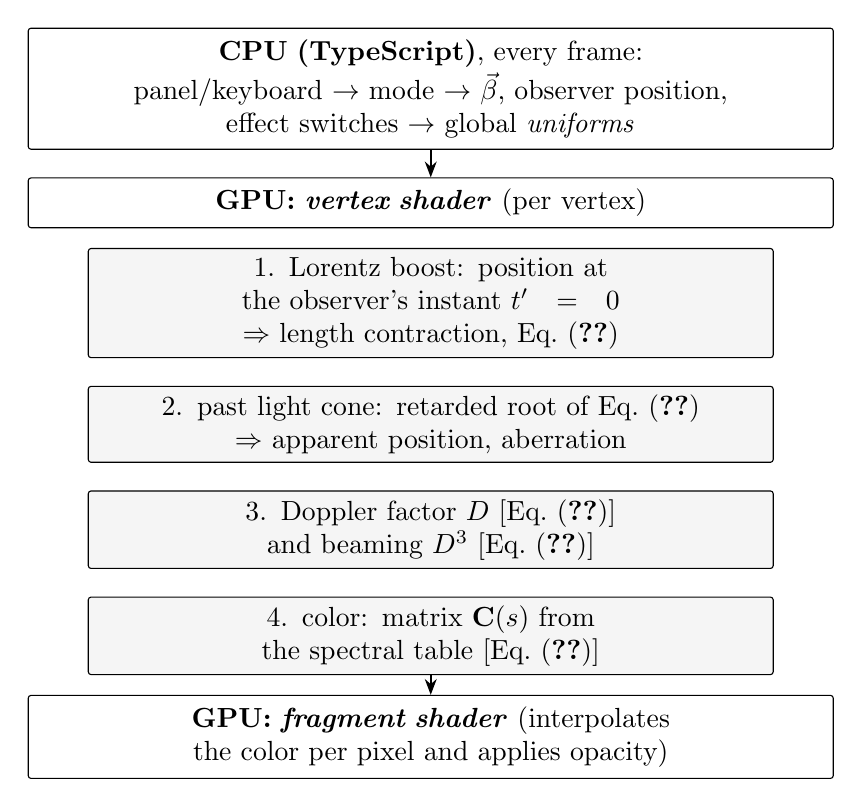
\begin{tikzpicture}[
      node distance=3.5mm,
      caixa/.style={draw, rounded corners=1pt, align=center, inner sep=4pt,
                    text width=0.82\columnwidth},
      etapa/.style={draw, rounded corners=1pt, align=center, inner sep=3pt,
                    text width=0.70\columnwidth, fill=black!4},
      seta/.style={-{Stealth[length=2mm]}, thick}
    ]
    \node[caixa] (cpu) {\textbf{CPU (TypeScript)}, every frame:\\[1pt]
      panel/keyboard $\to$ mode $\to$ $\vec{\beta}$, observer position,\\
      effect switches $\to$ global \emph{uniforms}};
    \node[caixa, below=of cpu] (vs) {\textbf{GPU: \emph{vertex shader}} (per vertex)};
    \node[etapa, below=2.5mm of vs] (e1) {1. Lorentz boost: position at the observer's
      instant $t'=0$\\ $\Rightarrow$ length contraction,
      Eq.~\eqref{eq:contracao}};
    \node[etapa, below=of e1] (e2) {2. past light cone: retarded root of
      Eq.~\eqref{eq:quadratica}\\ $\Rightarrow$ apparent position, aberration};
    \node[etapa, below=of e2] (e3) {3. Doppler factor $D$ [Eq.~\eqref{eq:doppler}] and
      beaming $D^{3}$ [Eq.~\eqref{eq:beaming}]};
    \node[etapa, below=of e3] (e4) {4. color: matrix $\mathbf{C}(s)$ from the spectral table
      [Eq.~\eqref{eq:cormatriz}]};
    \node[caixa, below=2.5mm of e4] (fs) {\textbf{GPU: \emph{fragment shader}}
      (interpolates the color per pixel and applies opacity)};
    \draw[seta] (cpu) -- (vs);
    \draw[seta] (e4) -- (fs);
  \end{tikzpicture}
  \caption{Pipeline of one frame: the CPU prepares a few values per frame and the GPU
           recomputes the apparent position and the color of every vertex of every
           object.}
  \label{fig:pipeline}
\end{figure}

\subsection{The per-vertex algorithm}

The vertex shader executes, for each vertex, four steps in sequence.

\paragraph{Step 1: Lorentz boost and contraction.} The vertex position is translated to a
frame with the observer at the origin. Next, the position of the object \emph{at the
observer's present instant} is sought, that is, at $t' = 0$ of the frame moving with
$\vec{\beta}$. Imposing $t' = 0$ on the time transformation of Eq.~\eqref{eq:lorentz}
applied to the vertex world line gives the laboratory instant
\begin{equation}
  T_{p} = \frac{\vec{\beta}\cdot\vec{x}_{\mathrm{lab}}}
               {1 - \vec{\beta}\cdot\vec{\beta}_{\mathrm{obj}}},
  \label{eq:tp}
\end{equation}
and the spatial boost, decomposed along directions parallel and perpendicular to
$\hat{\beta}$, leads to the position
\begin{equation}
  \begin{aligned}
    \vec{r}_{0} &= \vec{X} + (\gamma - 1)\,(\hat{\beta}\cdot\vec{X})\,\hat{\beta}
                   - \gamma\,\vec{\beta}\,T_{p},\\
    \vec{X} &= \vec{x}_{\mathrm{lab}} + \vec{\beta}_{\mathrm{obj}}\,T_{p}.
  \end{aligned}
  \label{eq:boost}
\end{equation}
The contraction arises from the simultaneity slice: since $T_{p}$ varies from vertex to
vertex (relativity of simultaneity), the combination of the boost with the evaluation of
each vertex at its own $T_{p}$ reduces the parallel coordinate of an object at rest in
the laboratory to $x_{\parallel}/\gamma$, which is exactly the contraction of
Eq.~\eqref{eq:contracao} appearing on screen. The velocity of the object as seen by the
observer is composed with Eq.~\eqref{eq:veladd}.

\paragraph{Step 2: apparent position.} With the aberration effect enabled, the shader
solves the quadratic of Eq.~\eqref{eq:quadratica} and selects the physical root
$\tau \leq 0$; for $|\vec{u}| < 1$ the two roots always have opposite signs and the
choice is unambiguous. The vertex is displaced to the apparent position of
Eq.~\eqref{eq:aparente}; numerical guards handle the nearly linear case
($|\vec{u}|^{2} \approx 1$, where the quadratic degenerates).

\paragraph{Step 3: Doppler and beaming.} The line of sight
$\hat{n} = \vec{r}_{\mathrm{ap}}/|\vec{r}_{\mathrm{ap}}|$ is defined and the factor $D$
of Eq.~\eqref{eq:doppler} is computed with the velocity of the object relative to the
observer (composed in Step 1) and the corresponding $\gamma$. Brightness is multiplied by
$D^{3}$ when beaming is enabled.

\paragraph{Step 4: color.} The rest color goes through the spectral reconstruction of
Section~\ref{sec:cor}, with the shift $\lambda_{\mathrm{obs}} =
\lambda_{\mathrm{emit}}/D$, and the result is interpolated by rasterization down to the
fragment shader, which is limited to applying opacity.

Each effect (contraction, aberration, Doppler, beaming) is controlled by its own switch
in the panel, passed to the shader as a $0/1$ uniform (a linear mix in the case of
contraction, a conditional branch for the others). This way, the student can enable one
effect at a time and identify the contribution of each term of the equations.

\subsection{Computational cost: per vertex versus per pixel}

The spectral reconstruction is a numerical integral over the visible band, far too
expensive to evaluate in real time. The engineering choice was to move it entirely out of
the rendering loop: since Eq.~\eqref{eq:cormatriz} shows that the result depends on a
single scalar parameter $s$, the integral is solved on the CPU at start-up and tabulated.
What remains in the shader is a texture lookup and a matrix-vector product, with no
exponentials.

The second choice is \emph{where} to pay the residual cost: per \emph{pixel} (millions of
evaluations per frame at full screen) or per \emph{vertex} (typically orders of magnitude
fewer evaluations), with the graphics card linearly interpolating the result along each
triangle, in the style of Gouraud shading. Per-vertex computation was adopted, decisive
for keeping interactivity on modest GPUs. The price is the possibility of interpolation
artifacts on coarse meshes; the mitigation is geometric: the scene meshes are subdivided
enough that the color variation between neighboring vertices is small. In addition, a
quality selector adjusts the renderer's device pixel ratio, reducing the number of
rasterized fragments on slow machines.

\subsection{Observation modes}

Three modes, selectable in the panel, define how the $\vec{\beta}$ vector and the camera
are built every frame:

\begin{enumerate}
  \item \textbf{Laboratory (orbital):} external orbital camera; the conceptual observer
        is at the origin and $\vec{\beta}$ is assembled from a magnitude slider and a
        chosen axis. It is the ideal mode to see, from the outside, the contraction and
        the apparent deformation of the scene. Presets fix $\gamma = 2$, $5$ and $10$ via
        $\beta = \sqrt{1 - 1/\gamma^{2}}$.
  \item \textbf{Observer's eye:} the observer stays still at the origin and
        \emph{$\vec{\beta}$ follows the gaze direction}: turning the eye rotates the
        direction of motion and, with it, the blue-shifted region (ahead) and the
        red-shifted region (behind).
  \item \textbf{First person:} keyboard navigation (WASD) with constant velocity: at
        every instant the observer occupies a well-defined inertial frame, consistent
        with the Physics 4 scope, with no relativistic acceleration phase.
\end{enumerate}

In every mode the magnitude is saturated ($|\vec{\beta}| \leq 0.9999$) to avoid
$\gamma \to \infty$, and a readout panel (HUD) displays $\beta$, $\gamma$,
$L/L_{0} = 1/\gamma$, the dilation factor, the frame rate (FPS) and two analog clocks,
one for the laboratory and one for the observer, integrated with $d\tau = dt/\gamma$,
which makes time dilation visible in real time. The interface is available in Portuguese
and English, selectable in the control panel.

\section{Results}

\subsection{Observable effects}

Figure~\ref{fig:repouso} shows the reference scene at rest ($\beta = 0$): a grid floor, a
horizontal ruler and a gallery of colored solids. In it, the two HUD clocks advance
together ($\gamma = 1$).

\begin{figure}[t]
  \centering
  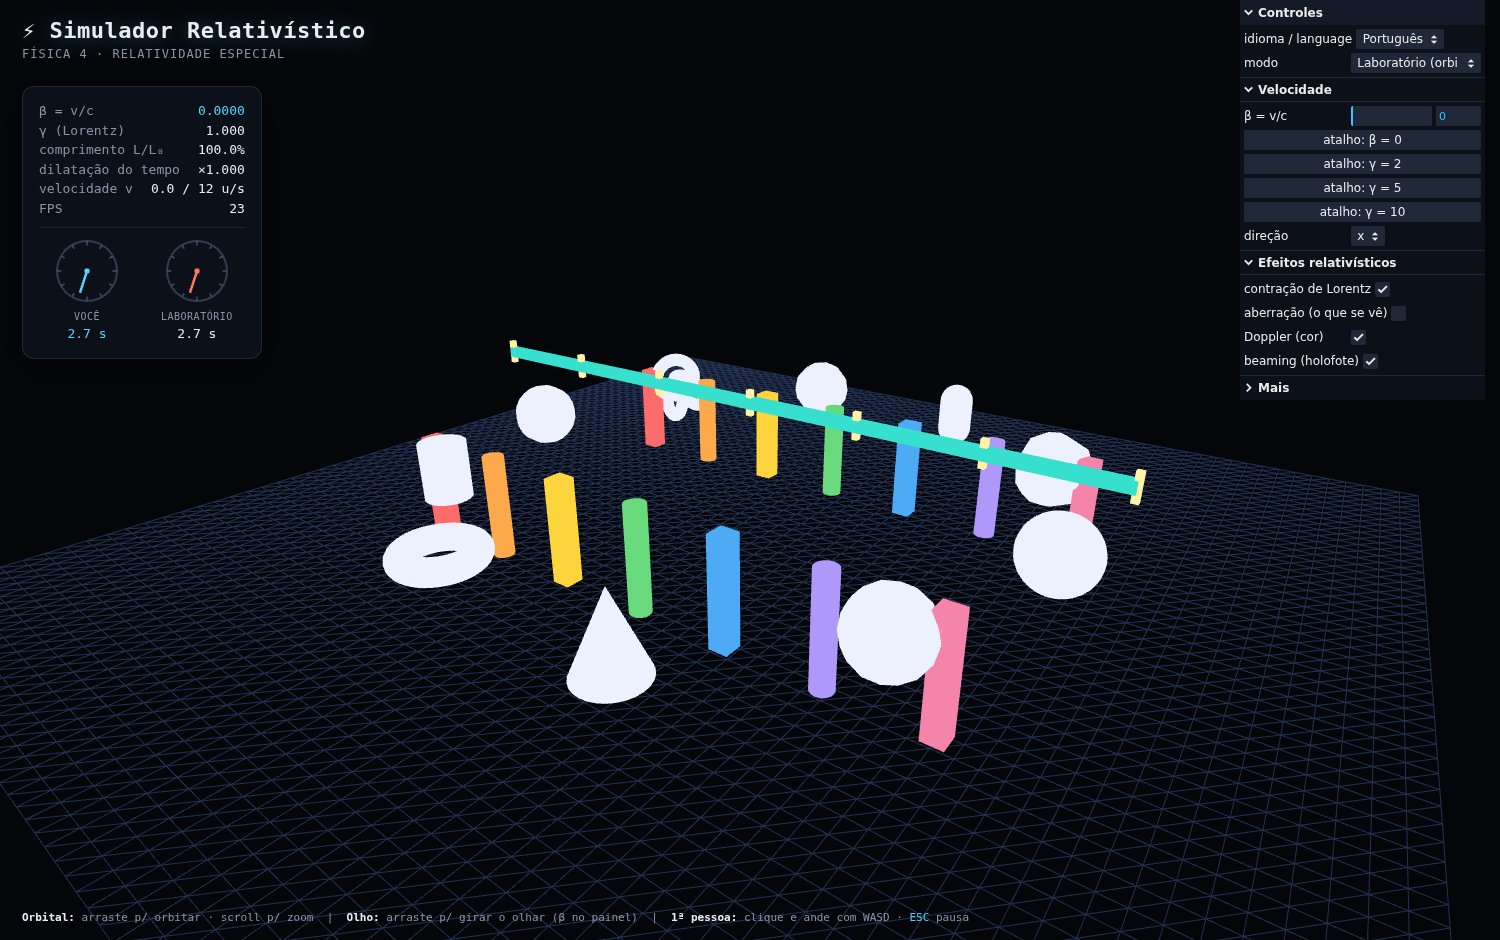
\includegraphics[width=\columnwidth]{figuras/en/lab-repouso.png}
  \caption{Laboratory scene at rest ($\beta = 0$, $\gamma = 1$): original geometry and
           colors; the two HUD clocks advance at the same rate.}
  \label{fig:repouso}
\end{figure}

With $\beta = 0.7$ along the $x$ axis (Figure~\ref{fig:beta07}), the following appear
simultaneously: the contraction of the shapes along the direction of motion
($L/L_{0} = 71.4\%$, HUD); the Doppler shift, with objects blue-shifted in the approach
direction, red-shifted in the opposite one and the floor displaying the continuous color
gradient along the line of sight; beaming, which darkens the recession region; and time
dilation on the clocks ($3.5$~s of proper time against $4.9$~s of laboratory time, factor
$\times 1.400 = \gamma$).

\begin{figure}[t]
  \centering
  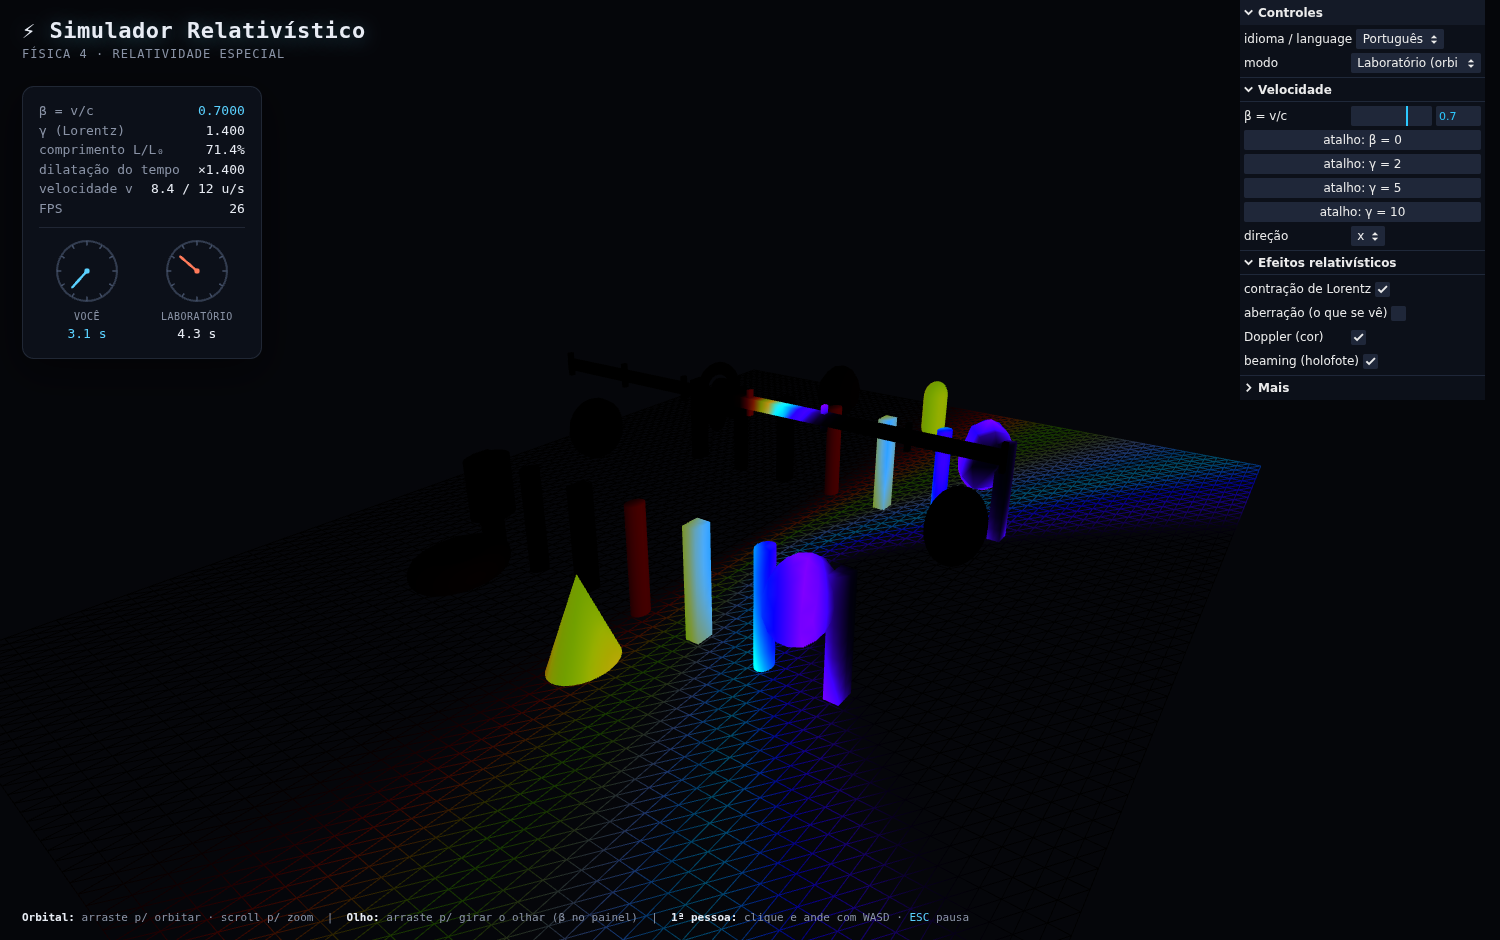
\includegraphics[width=\columnwidth]{figuras/en/lab-beta07.png}
  \caption{Same scene with $\beta = 0.7$: contraction ($L/L_{0} = 71.4\%$), Doppler and
           beaming; the clocks display the dilation $\gamma = 1.4$.}
  \label{fig:beta07}
\end{figure}

Enabling the apparent position (Figure~\ref{fig:aberracao}), the retarded time of
Eq.~\eqref{eq:quadratica} displaces each vertex individually: straight columns appear
bent and the solids, rotated. It is the manifestation, for extended objects, of the
Terrell--Penrose rotation, and the direct visual difference between \emph{what is
measured} (Figure~\ref{fig:beta07}) and \emph{what is seen}
(Figure~\ref{fig:aberracao}).

\begin{figure}[t]
  \centering
  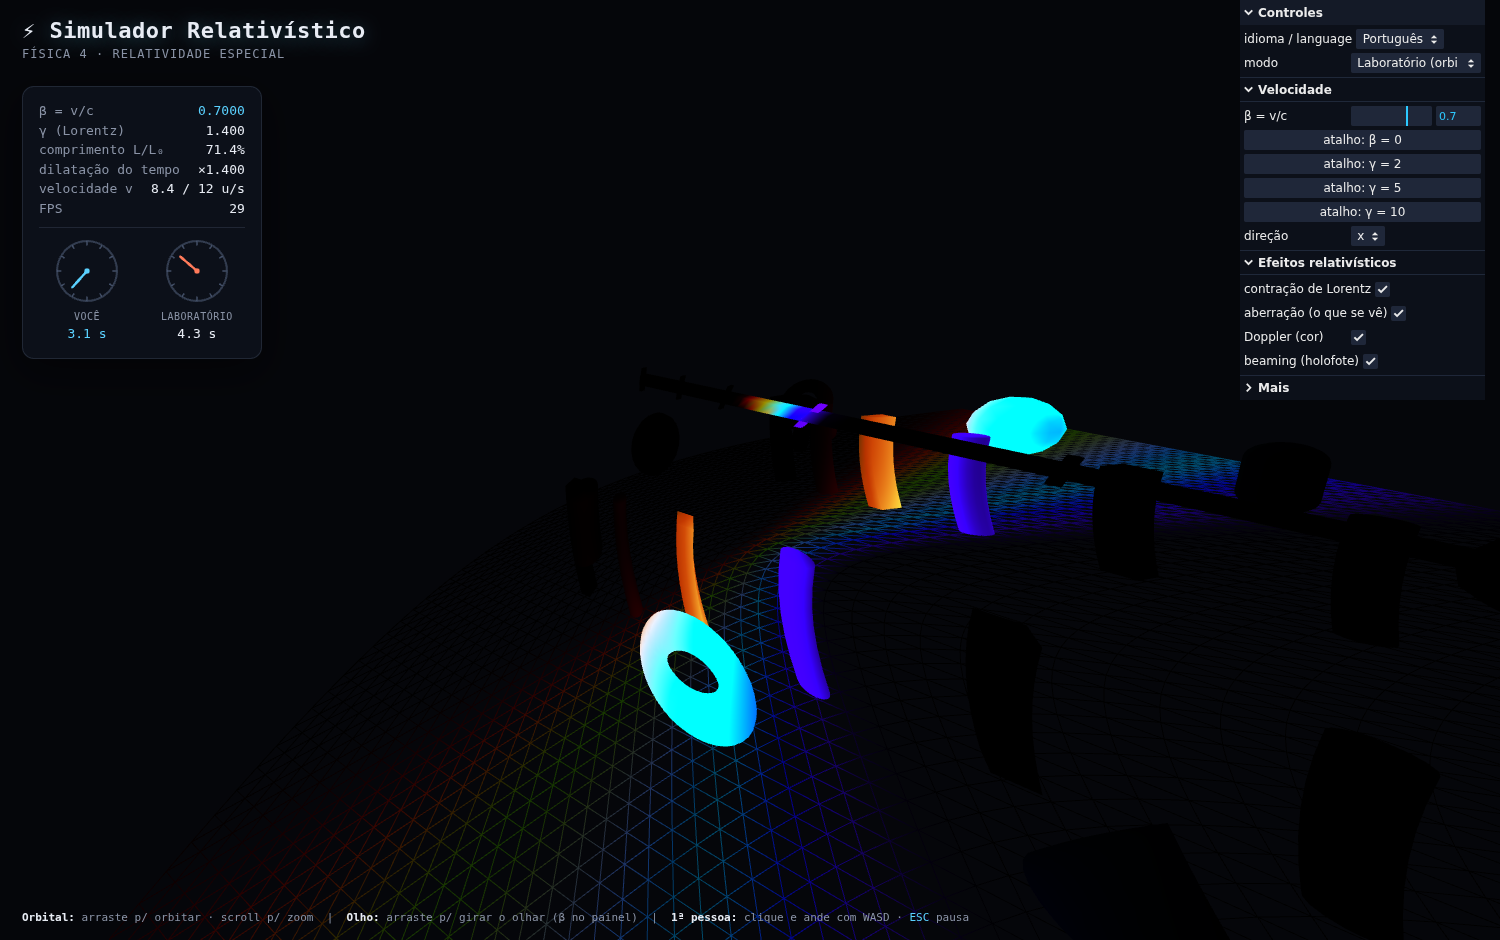
\includegraphics[width=\columnwidth]{figuras/en/lab-aberracao.png}
  \caption{$\beta = 0.7$ with apparent position (past light cone) enabled: straight
           columns appear bent and the solids rotated (Terrell--Penrose).}
  \label{fig:aberracao}
\end{figure}

In the Observer's Eye mode (Figure~\ref{fig:olho}), the observer standing at the origin
``looks'' along their own direction of motion: even at $\beta = 0.25$ the blueshift ahead
is clear, with the color gradient sweeping continuously across the scene as the line of
sight moves away from the direction of motion.

\begin{figure}[t]
  \centering
  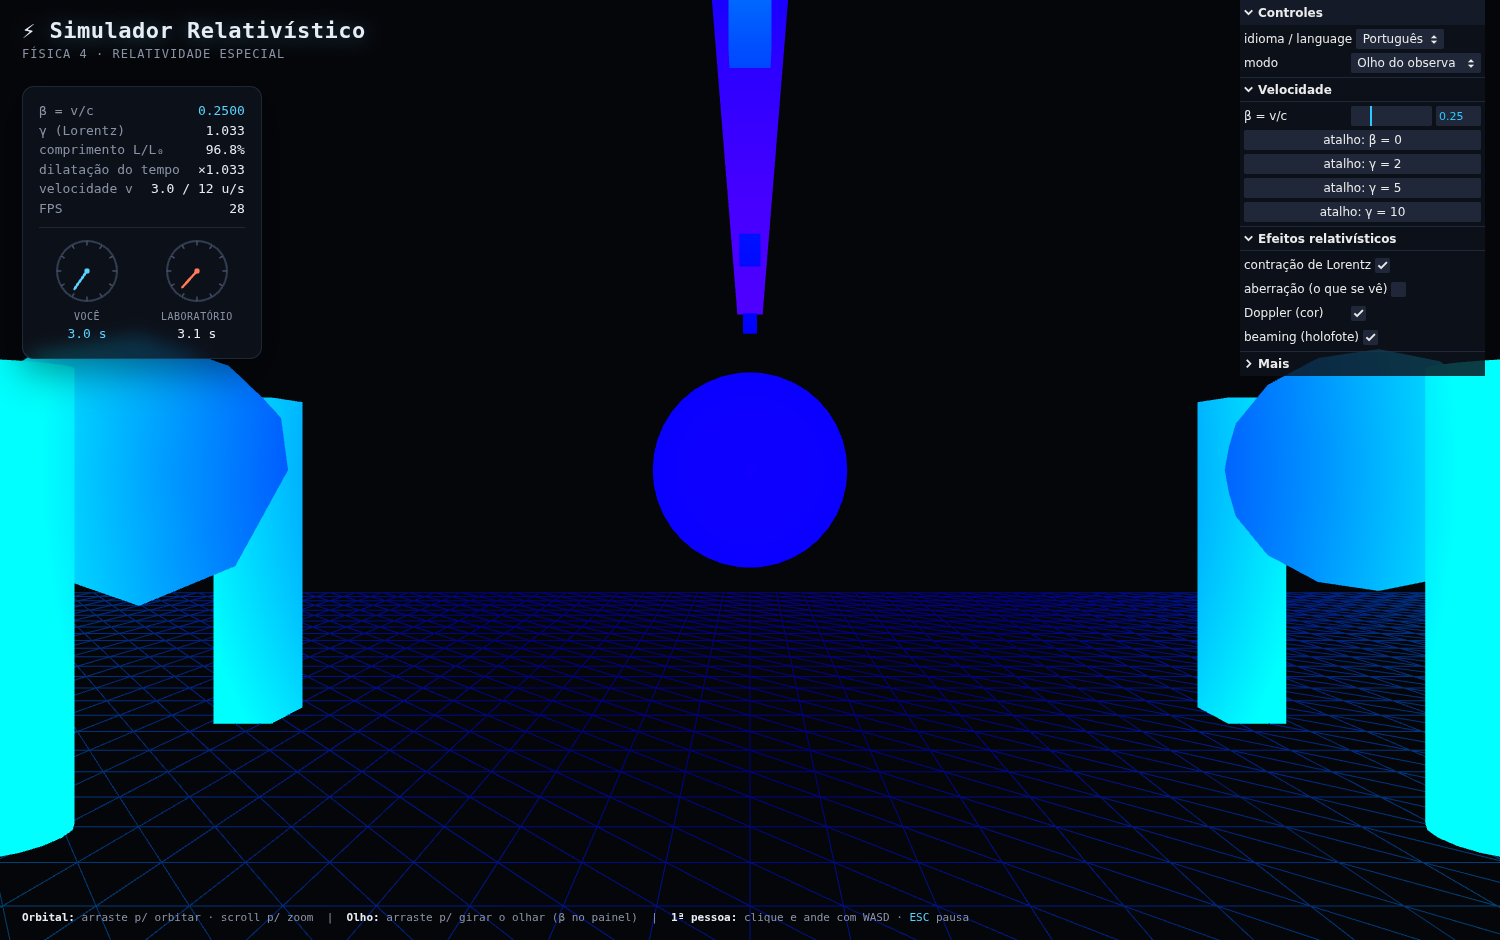
\includegraphics[width=\columnwidth]{figuras/en/olho-beta025.png}
  \caption{Observer's Eye mode, $\beta = 0.25$ along the gaze direction: blueshift ahead,
           with a continuous color gradient across the scene.}
  \label{fig:olho}
\end{figure}

At $\beta = 0.9$ (Figure~\ref{fig:beta09}), the spectral shift is so intense that the
visible light of several objects leaves the perceptible band and they darken, a predicted
consequence of the color model without spectral reserve (Section~\ref{sec:cor}): the
intense blue disappears into the ultraviolet ahead and the red, into the infrared behind.

\begin{figure}[t]
  \centering
  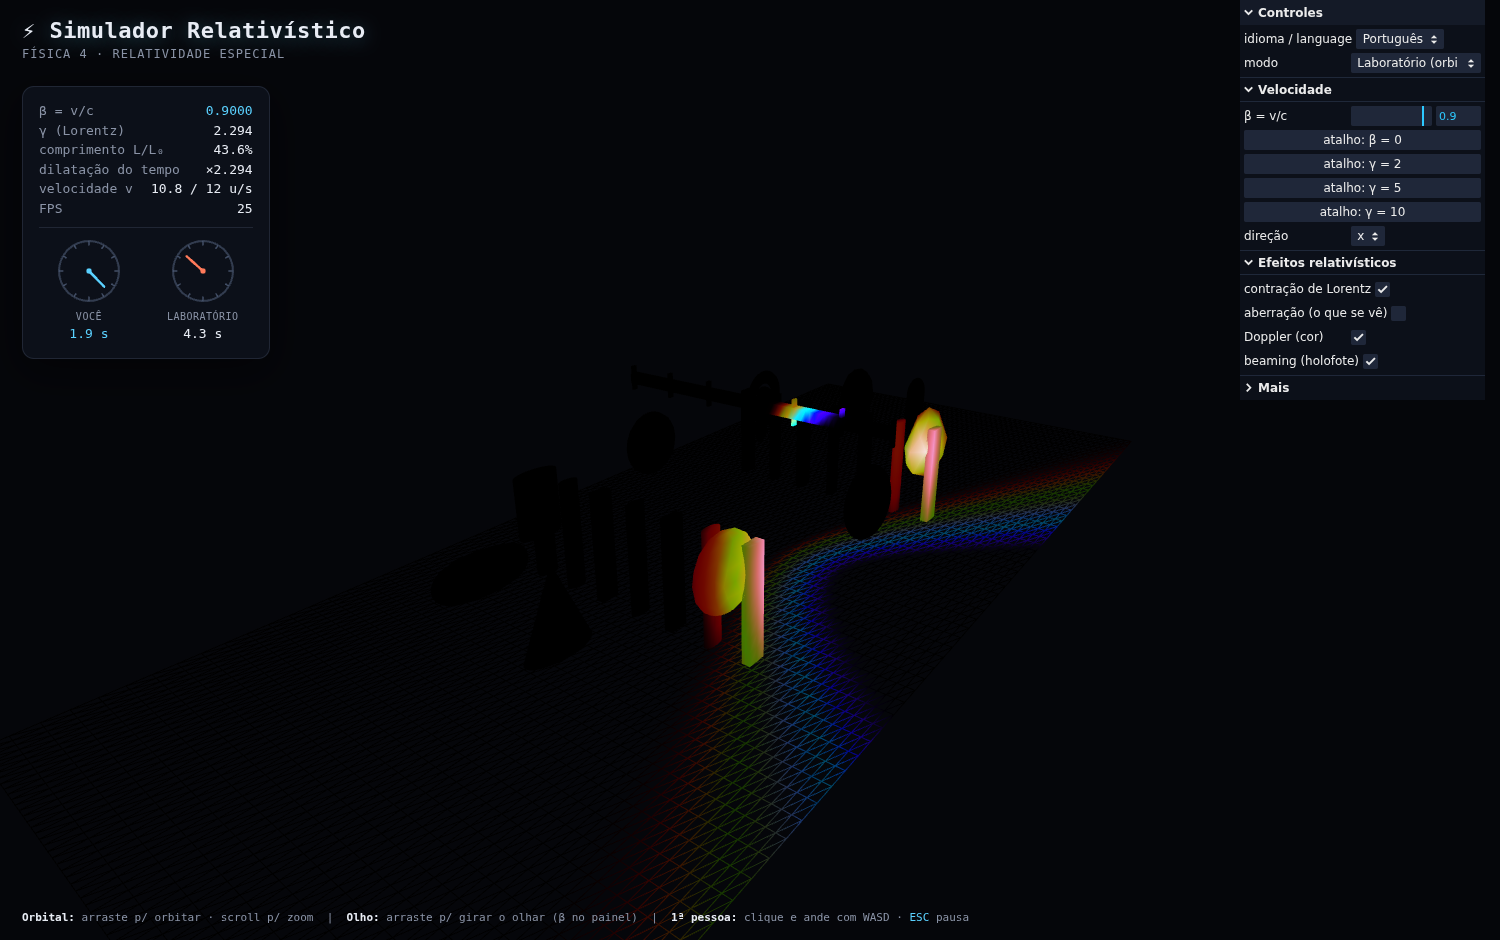
\includegraphics[width=\columnwidth]{figuras/en/lab-beta09.png}
  \caption{$\beta = 0.9$ ($\gamma = 2.294$): objects darken when their visible light is
           shifted outside the perceptible band, the expected behavior of the
           band-limited color model.}
  \label{fig:beta09}
\end{figure}

\subsection{Performance}

By concentrating the physics in the vertex shader and keeping the fragment shader
trivial, the simulation sustains interactive rates (tens of frames per second) even under
software rendering, without a dedicated GPU; the figure captures, taken under those
conditions, register between 23 and 28~FPS on the HUD. On common hardware with graphics
acceleration, the rate is limited by the display refresh. The quality selector reduces
the renderer's pixel ratio when needed, and the HUD frame-rate meter lets the user
calibrate the adjustment.

\subsection{Limitations and simplifications}
\label{sec:limitacoes}

Table~\ref{tab:limitacoes} consolidates the adopted simplifications, their nature and the
main effect of each one. Two of them deserve comment. The color model does not reserve
energy in the infrared/ultraviolet: at high $\beta$, objects darken instead of displaying
the brightness that a real broad-spectrum source would keep, although the qualitative
behavior of the shift (blueing/reddening) remains correct. In addition, the scope is
restricted to constant velocity: the transformations applied at each frame are rigorously
correct for the instantaneous inertial frame, but velocity changes are idealized, with no
continuous acceleration phase and none of the associated phenomena, such as Thomas
precession, a restriction aligned with the Physics 4 level.

\begin{table}[t]
  \centering
  \caption{Main simplifications of the model and their effects.}
  \label{tab:limitacoes}
  \footnotesize
  \setlength{\tabcolsep}{3pt}
  \begin{tabular}{@{}>{\raggedright\arraybackslash}p{0.34\columnwidth}%
                     >{\raggedright\arraybackslash}p{0.19\columnwidth}%
                     >{\raggedright\arraybackslash}p{0.38\columnwidth}@{}}
    \toprule
    Simplification & Nature & Main effect \\
    \midrule
    Color without IR/UV reserve  & color model  & darkening at high $\beta$ \\
    No lighting/shadows          & rendering    & self-luminous appearance \\
    Constant velocity            & scope (SR)   & no relativistic acceleration \\
    Per-vertex color (Gouraud)   & performance  & artifacts on coarse meshes \\
    Arbitrary units, adjustable $c$ & didactics & only ratios ($\beta$, $\gamma$, $D$) faithful \\
    \bottomrule
  \end{tabular}
\end{table}

\subsection{Availability}

The simulator is published and can be run in any modern browser, with no installation:
\begin{center}\small
  \url{https://sergiomaccari.github.io/Simulador-Relativ-stico/}
\end{center}
The complete source code (TypeScript, GLSL and this document) is available at:
\begin{center}\small
  \url{https://github.com/sergiomaccari/Simulador-Relativ-stico}
\end{center}
For local execution, \texttt{npm install} and \texttt{npm run dev} at the repository root
are enough.

\section{Conclusion}

The developed simulator demonstrates that the optical effects of Special Relativity
(Lorentz contraction, time dilation, aberration via the past light cone, the relativistic
Doppler effect and beaming) can be visualized in an interactive, quantitative and
physically grounded way in an open web application, with no installation. The per-vertex
GPU implementation proved sufficient to keep interactivity even without dedicated
graphics acceleration. The individual switches for each effect, together with the
explicit distinction between \emph{measuring} (Lorentz transformation) and \emph{seeing}
(retarded time), give the student a visual laboratory in which every term of the
canonical equations has an observable counterpart on screen. Natural extensions include
the spectral reserve in the infrared/ultraviolet in the color model, per-fragment Doppler
computation and an advanced mode with accelerated (hyperbolic) motion, the latter already
outside the scope of Physics 4.

\begin{referencias}
  \item Einstein, A. (1905). Zur Elektrodynamik bewegter Körper. \emph{Annalen der
        Physik}, 17, 891--921.
  \item Griffiths, D.J. (2017). \emph{Introduction to Electrodynamics}. 4th ed.
        Cambridge University Press, Cambridge.
  \item Kortemeyer, G., Tan, P. and Schirra, S. (2013). A Slower Speed of Light:
        developing intuition about special relativity with games. In \emph{Proceedings of
        the 8th International Conference on the Foundations of Digital Games (FDG 2013)},
        400--402. SASDG, Chania, Greece.
  \item Michelson, A.A. and Morley, E.W. (1887). On the relative motion of the Earth and
        the luminiferous ether. \emph{American Journal of Science}, 34, 333--345.
  \item MIT Game Lab (2013). \emph{OpenRelativity} [computer software]. Massachusetts
        Institute of Technology. MIT License.
        \url{https://github.com/MITGameLab/OpenRelativity}.
  \item Nussenzveig, H.M. (2014). \emph{Curso de Física Básica, vol. 4: Ótica,
        Relatividade, Física Quântica}. 2nd ed. Blucher, São Paulo.
  \item Penrose, R. (1959). The apparent shape of a relativistically moving sphere.
        \emph{Proceedings of the Cambridge Philosophical Society}, 55(1), 137--139.
  \item Sherin, Z.W., Cheu, R., Tan, P. and Kortemeyer, G. (2016). Visualizing relativity:
        the OpenRelativity project. \emph{American Journal of Physics}, 84(5), 369--374.
  \item Terrell, J. (1959). Invisibility of the Lorentz contraction. \emph{Physical
        Review}, 116(4), 1041--1045.
  \item Wyman, C., Sloan, P.-P. and Shirley, P. (2013). Simple analytic approximations to
        the CIE XYZ color matching functions. \emph{Journal of Computer Graphics
        Techniques}, 2(2), 1--11.
\end{referencias}

\end{document}
